% Options for packages loaded elsewhere
\PassOptionsToPackage{unicode}{hyperref}
\PassOptionsToPackage{hyphens}{url}
%
\documentclass[
]{article}
\usepackage{lmodern}
\usepackage{amssymb,amsmath}
\usepackage{ifxetex,ifluatex}
\ifnum 0\ifxetex 1\fi\ifluatex 1\fi=0 % if pdftex
  \usepackage[T1]{fontenc}
  \usepackage[utf8]{inputenc}
  \usepackage{textcomp} % provide euro and other symbols
\else % if luatex or xetex
  \usepackage{unicode-math}
  \defaultfontfeatures{Scale=MatchLowercase}
  \defaultfontfeatures[\rmfamily]{Ligatures=TeX,Scale=1}
\fi
% Use upquote if available, for straight quotes in verbatim environments
\IfFileExists{upquote.sty}{\usepackage{upquote}}{}
\IfFileExists{microtype.sty}{% use microtype if available
  \usepackage[]{microtype}
  \UseMicrotypeSet[protrusion]{basicmath} % disable protrusion for tt fonts
}{}
\makeatletter
\@ifundefined{KOMAClassName}{% if non-KOMA class
  \IfFileExists{parskip.sty}{%
    \usepackage{parskip}
  }{% else
    \setlength{\parindent}{0pt}
    \setlength{\parskip}{6pt plus 2pt minus 1pt}}
}{% if KOMA class
  \KOMAoptions{parskip=half}}
\makeatother
\usepackage{xcolor}
\IfFileExists{xurl.sty}{\usepackage{xurl}}{} % add URL line breaks if available
\IfFileExists{bookmark.sty}{\usepackage{bookmark}}{\usepackage{hyperref}}
\hypersetup{
  pdftitle={stad80A1},
  pdfauthor={Zi Jian Liu},
  hidelinks,
  pdfcreator={LaTeX via pandoc}}
\urlstyle{same} % disable monospaced font for URLs
\usepackage[margin=1in]{geometry}
\usepackage{color}
\usepackage{fancyvrb}
\newcommand{\VerbBar}{|}
\newcommand{\VERB}{\Verb[commandchars=\\\{\}]}
\DefineVerbatimEnvironment{Highlighting}{Verbatim}{commandchars=\\\{\}}
% Add ',fontsize=\small' for more characters per line
\usepackage{framed}
\definecolor{shadecolor}{RGB}{248,248,248}
\newenvironment{Shaded}{\begin{snugshade}}{\end{snugshade}}
\newcommand{\AlertTok}[1]{\textcolor[rgb]{0.94,0.16,0.16}{#1}}
\newcommand{\AnnotationTok}[1]{\textcolor[rgb]{0.56,0.35,0.01}{\textbf{\textit{#1}}}}
\newcommand{\AttributeTok}[1]{\textcolor[rgb]{0.77,0.63,0.00}{#1}}
\newcommand{\BaseNTok}[1]{\textcolor[rgb]{0.00,0.00,0.81}{#1}}
\newcommand{\BuiltInTok}[1]{#1}
\newcommand{\CharTok}[1]{\textcolor[rgb]{0.31,0.60,0.02}{#1}}
\newcommand{\CommentTok}[1]{\textcolor[rgb]{0.56,0.35,0.01}{\textit{#1}}}
\newcommand{\CommentVarTok}[1]{\textcolor[rgb]{0.56,0.35,0.01}{\textbf{\textit{#1}}}}
\newcommand{\ConstantTok}[1]{\textcolor[rgb]{0.00,0.00,0.00}{#1}}
\newcommand{\ControlFlowTok}[1]{\textcolor[rgb]{0.13,0.29,0.53}{\textbf{#1}}}
\newcommand{\DataTypeTok}[1]{\textcolor[rgb]{0.13,0.29,0.53}{#1}}
\newcommand{\DecValTok}[1]{\textcolor[rgb]{0.00,0.00,0.81}{#1}}
\newcommand{\DocumentationTok}[1]{\textcolor[rgb]{0.56,0.35,0.01}{\textbf{\textit{#1}}}}
\newcommand{\ErrorTok}[1]{\textcolor[rgb]{0.64,0.00,0.00}{\textbf{#1}}}
\newcommand{\ExtensionTok}[1]{#1}
\newcommand{\FloatTok}[1]{\textcolor[rgb]{0.00,0.00,0.81}{#1}}
\newcommand{\FunctionTok}[1]{\textcolor[rgb]{0.00,0.00,0.00}{#1}}
\newcommand{\ImportTok}[1]{#1}
\newcommand{\InformationTok}[1]{\textcolor[rgb]{0.56,0.35,0.01}{\textbf{\textit{#1}}}}
\newcommand{\KeywordTok}[1]{\textcolor[rgb]{0.13,0.29,0.53}{\textbf{#1}}}
\newcommand{\NormalTok}[1]{#1}
\newcommand{\OperatorTok}[1]{\textcolor[rgb]{0.81,0.36,0.00}{\textbf{#1}}}
\newcommand{\OtherTok}[1]{\textcolor[rgb]{0.56,0.35,0.01}{#1}}
\newcommand{\PreprocessorTok}[1]{\textcolor[rgb]{0.56,0.35,0.01}{\textit{#1}}}
\newcommand{\RegionMarkerTok}[1]{#1}
\newcommand{\SpecialCharTok}[1]{\textcolor[rgb]{0.00,0.00,0.00}{#1}}
\newcommand{\SpecialStringTok}[1]{\textcolor[rgb]{0.31,0.60,0.02}{#1}}
\newcommand{\StringTok}[1]{\textcolor[rgb]{0.31,0.60,0.02}{#1}}
\newcommand{\VariableTok}[1]{\textcolor[rgb]{0.00,0.00,0.00}{#1}}
\newcommand{\VerbatimStringTok}[1]{\textcolor[rgb]{0.31,0.60,0.02}{#1}}
\newcommand{\WarningTok}[1]{\textcolor[rgb]{0.56,0.35,0.01}{\textbf{\textit{#1}}}}
\usepackage{graphicx,grffile}
\makeatletter
\def\maxwidth{\ifdim\Gin@nat@width>\linewidth\linewidth\else\Gin@nat@width\fi}
\def\maxheight{\ifdim\Gin@nat@height>\textheight\textheight\else\Gin@nat@height\fi}
\makeatother
% Scale images if necessary, so that they will not overflow the page
% margins by default, and it is still possible to overwrite the defaults
% using explicit options in \includegraphics[width, height, ...]{}
\setkeys{Gin}{width=\maxwidth,height=\maxheight,keepaspectratio}
% Set default figure placement to htbp
\makeatletter
\def\fps@figure{htbp}
\makeatother
\setlength{\emergencystretch}{3em} % prevent overfull lines
\providecommand{\tightlist}{%
  \setlength{\itemsep}{0pt}\setlength{\parskip}{0pt}}
\setcounter{secnumdepth}{-\maxdimen} % remove section numbering

\title{stad80A1}
\author{Zi Jian Liu}
\date{1/25/2021}

\begin{document}
\maketitle

{
\setcounter{tocdepth}{2}
\tableofcontents
}
\hypertarget{section}{%
\section{1.}\label{section}}

\hypertarget{section-1}{%
\subsection{(1)}\label{section-1}}

Wrong statements: C. E.\\
\#\# (2)\\
Wrong statements: A. B. C.\\
\#\# (3)\\
Wrong statements: C. \#\# (4)\\
Wrong statements: A.\\
\#\# (5)\\
Correct statements: B. D.\\
\#\# (6)\\
Wrong statements: c.~E.

\hypertarget{section-2}{%
\section{2.}\label{section-2}}

\hypertarget{a}{%
\subsection{2.a)}\label{a}}

\[l(\theta )=\sum_{i=1}^{n}(log(\theta -1)-\theta log(X_{i})) \\
= nlog(\theta -1) - \theta \sum_{i=1}^{n}logX_{i} \\
\Rightarrow \frac{\partial }{\partial \theta } = \frac{n}{\theta -1}-\sum_{i=1}^{n}logX_{i} = 0 \\
n = \sum log X_{i} (\theta -1) \\
\Rightarrow \hat\theta_{n} = \frac{n}{\sum log X_{i}} + 1 \\
= \frac{1}{\bar{log X_{i}}} + 1 \\\]\\
\#\# 2.b)\\
\[I(\theta ) = -\int_{1}^{\infty }(\frac{\partial^2 }{\partial \theta ^2}log((\theta -1)x^{-\theta } ))(\theta -1)x^{-\theta }dx \\
= -\int_{1}^{\infty }(\frac{\partial }{\partial \theta }\frac{1}{(\theta -1)}-logx)(\theta -1)x^{-\theta }dx \\
= \int_{1}^{\infty }(\frac{1}{(\theta -1)})x^{-\theta }dx \\
=\int_{1}^{\infty }\frac{x^{-\theta }}{\theta -1}dx \\
=0 + \frac{1^{1-\theta }}{(\theta -1)^{2}} \\
=\frac{1}{(\theta -1)^{2}} \\\\\]\[
(\hat{\theta _{n}}-\theta ) \overset{d}{\rightarrow} N(0,\frac{1}{nI(\theta )}) \\
\Rightarrow \lim_{n\rightarrow \infty }\frac{1}{nI(\theta )} = \lim_{n\rightarrow \infty }\frac{1}{n}(\theta -1)^{2} = 0 \\
\] \#\# 2.c)\\
\[C_{n} = [\hat{\theta _{n}}-\frac{z_{\alpha /2}}{\sqrt{nI(\hat{\theta _{n}})}}, \hat{\theta _{n}}+\frac{z_{\alpha /2}}{\sqrt{nI(\hat{\theta _{n}})}} ]\\
= [\hat{\theta _{n}}-\frac{z_{0.025}}{\sqrt{n(\frac{1}{(\theta -1)^{2}})}}, \hat{\theta _{n}}+\frac{z_{0.025}}{\sqrt{n(\frac{1}{(\theta -1)^{2}})}} ]\\
=[\frac{1}{\overline{logX_{i}}} + 1 - \frac{1.96}{n(\frac{1}{(\theta -1)^{2}})},\frac{1}{\overline{logX_{i}}} + 1 + \frac{1.96}{n(\frac{1}{(\theta -1)^{2}})}] \\\]

\hypertarget{d}{%
\subsection{2.d)}\label{d}}
\begin{equation} 
F(x) = \int_{1}^{\infty }(\theta -1)x^{-\theta }dx \\
= (-1 +y)(\frac{x^{-y+1}}{-y+1}-\frac{1}{-y+1}) \\
= (-1 +2 )(\frac{x^{-2 +1}}{-2 +1}-\frac{1}{-2 +1}) \\
= (\frac{x^{-1}}{-1} + 1) \\
= 1 - \frac{1}{x} \\
\Rightarrow F^{-1}(x) = -\frac{1}{x-1} \\
\end{equation}


\begin{Shaded}
\begin{Highlighting}[]
\KeywordTok{set.seed}\NormalTok{(}\DecValTok{1003643587}\NormalTok{)}
\NormalTok{N <-}\StringTok{ }\DecValTok{10000}
\NormalTok{n <-}\StringTok{ }\DecValTok{100}
\NormalTok{t <-}\StringTok{ }\DecValTok{2}
\NormalTok{invCDF <-}\StringTok{ }\ControlFlowTok{function}\NormalTok{(u, t) \{}
  \KeywordTok{return}\NormalTok{(}\OperatorTok{-}\DecValTok{1}\OperatorTok{/}\NormalTok{(u}\DecValTok{-1}\NormalTok{))}
\NormalTok{\}}
\end{Highlighting}
\end{Shaded}

confidence interval

\begin{Shaded}
\begin{Highlighting}[]
\NormalTok{lowerBound <-}\StringTok{ }\KeywordTok{c}\NormalTok{()}
\NormalTok{upperBound <-}\StringTok{ }\KeywordTok{c}\NormalTok{()}
\ControlFlowTok{for}\NormalTok{ (i }\ControlFlowTok{in} \DecValTok{1}\OperatorTok{:}\NormalTok{N) \{}
\NormalTok{  uni <-}\StringTok{ }\KeywordTok{runif}\NormalTok{(}\DecValTok{100}\NormalTok{, }\DecValTok{0}\NormalTok{, }\DecValTok{1}\NormalTok{)}
\NormalTok{  samp <-}\StringTok{ }\KeywordTok{c}\NormalTok{()}
  \ControlFlowTok{for}\NormalTok{ (j }\ControlFlowTok{in} \DecValTok{1}\OperatorTok{:}\DecValTok{100}\NormalTok{) \{}
\NormalTok{    samp <-}\StringTok{ }\KeywordTok{append}\NormalTok{(samp, }\KeywordTok{invCDF}\NormalTok{(uni[j], t), }\DataTypeTok{after =} \KeywordTok{length}\NormalTok{(samp))}
\NormalTok{  \}}
\NormalTok{  upperBound <-}\StringTok{ }\KeywordTok{append}\NormalTok{(upperBound, }\DecValTok{1} \OperatorTok{+}\StringTok{ }\DecValTok{1}\OperatorTok{/}\KeywordTok{mean}\NormalTok{(}\KeywordTok{log}\NormalTok{(samp)) }\OperatorTok{+}\StringTok{ }\FloatTok{1.96}\OperatorTok{/}\NormalTok{(}\KeywordTok{sqrt}\NormalTok{(n}\OperatorTok{*}\KeywordTok{mean}\NormalTok{(}\KeywordTok{log}\NormalTok{(samp))}\OperatorTok{^}\DecValTok{2}\NormalTok{)), }\DataTypeTok{after =} \KeywordTok{length}\NormalTok{(upperBound))}
\NormalTok{  lowerBound <-}\StringTok{ }\KeywordTok{append}\NormalTok{(lowerBound, }\DecValTok{1} \OperatorTok{+}\StringTok{ }\DecValTok{1}\OperatorTok{/}\KeywordTok{mean}\NormalTok{(}\KeywordTok{log}\NormalTok{(samp)) }\OperatorTok{-}\StringTok{ }\FloatTok{1.96}\OperatorTok{/}\NormalTok{(}\KeywordTok{sqrt}\NormalTok{(n}\OperatorTok{*}\KeywordTok{mean}\NormalTok{(}\KeywordTok{log}\NormalTok{(samp))}\OperatorTok{^}\DecValTok{2}\NormalTok{)), }\DataTypeTok{after =} \KeywordTok{length}\NormalTok{(lowerBound))}
\NormalTok{\}}
\end{Highlighting}
\end{Shaded}

check for theta in confidence intervals

\begin{Shaded}
\begin{Highlighting}[]
\NormalTok{lowerBound =}\StringTok{ }\KeywordTok{replace}\NormalTok{(lowerBound, lowerBound }\OperatorTok{<=}\StringTok{ }\NormalTok{t, }\DecValTok{1}\NormalTok{)}
\NormalTok{lowerBound =}\StringTok{ }\KeywordTok{replace}\NormalTok{(lowerBound, lowerBound }\OperatorTok{>}\StringTok{ }\NormalTok{t, }\DecValTok{0}\NormalTok{)}
\NormalTok{upperBound =}\StringTok{ }\KeywordTok{replace}\NormalTok{(upperBound, upperBound }\OperatorTok{<}\StringTok{ }\NormalTok{t, }\DecValTok{0}\NormalTok{)}
\NormalTok{upperBound =}\StringTok{ }\KeywordTok{replace}\NormalTok{(upperBound, upperBound }\OperatorTok{>=}\StringTok{ }\NormalTok{t, }\DecValTok{1}\NormalTok{)}

\NormalTok{k <-}\StringTok{ }\DecValTok{0}
\ControlFlowTok{for}\NormalTok{ (l }\ControlFlowTok{in} \DecValTok{1}\OperatorTok{:}\NormalTok{N) \{}
  \ControlFlowTok{if}\NormalTok{(upperBound[l] }\OperatorTok{==}\StringTok{ }\DecValTok{1} \OperatorTok{&}\StringTok{ }\NormalTok{lowerBound[l] }\OperatorTok{==}\StringTok{ }\DecValTok{1}\NormalTok{) \{}
\NormalTok{    k <-}\StringTok{ }\NormalTok{k }\OperatorTok{+}\StringTok{ }\DecValTok{1}
\NormalTok{  \}}
\NormalTok{\}}
\KeywordTok{print}\NormalTok{(k}\OperatorTok{/}\NormalTok{N)}
\end{Highlighting}
\end{Shaded}

\begin{verbatim}
## [1] 0.9483
\end{verbatim}

As we can see, the frequency is 94.83\% which is really close to 95\%.
Therefore we can claim that the constructed CI is effective

\hypertarget{section-3}{%
\section{3.}\label{section-3}}

\hypertarget{a-1}{%
\subsection{3.a)}\label{a-1}}

\begin{Shaded}
\begin{Highlighting}[]
\KeywordTok{set.seed}\NormalTok{(}\DecValTok{1003643587}\NormalTok{)}
\NormalTok{N <-}\StringTok{ }\DecValTok{10}
\NormalTok{n <-}\StringTok{ }\KeywordTok{c}\NormalTok{(}\DecValTok{10}\NormalTok{,}\DecValTok{100}\NormalTok{,}\DecValTok{1000}\NormalTok{,}\DecValTok{10000}\NormalTok{)}

\CommentTok{# function that samples from uniform}
\NormalTok{samples <-}\StringTok{ }\ControlFlowTok{function}\NormalTok{(n) \{}
\NormalTok{  samplesReplaced =}\StringTok{ }\KeywordTok{runif}\NormalTok{(n, }\DataTypeTok{min =} \DecValTok{0}\NormalTok{, }\DataTypeTok{max =} \DecValTok{1}\NormalTok{)}
\NormalTok{  samplesReplaced =}\StringTok{ }\KeywordTok{replace}\NormalTok{(samplesReplaced, samplesReplaced}\OperatorTok{<}\FloatTok{0.5}\NormalTok{, }\DecValTok{-1}\NormalTok{)}
\NormalTok{  samplesReplaced =}\StringTok{ }\KeywordTok{replace}\NormalTok{(samplesReplaced, samplesReplaced}\OperatorTok{>=}\StringTok{ }\FloatTok{0.5}\NormalTok{, }\DecValTok{1}\NormalTok{)}
  \KeywordTok{return}\NormalTok{(samplesReplaced)}
\NormalTok{\}}
\end{Highlighting}
\end{Shaded}

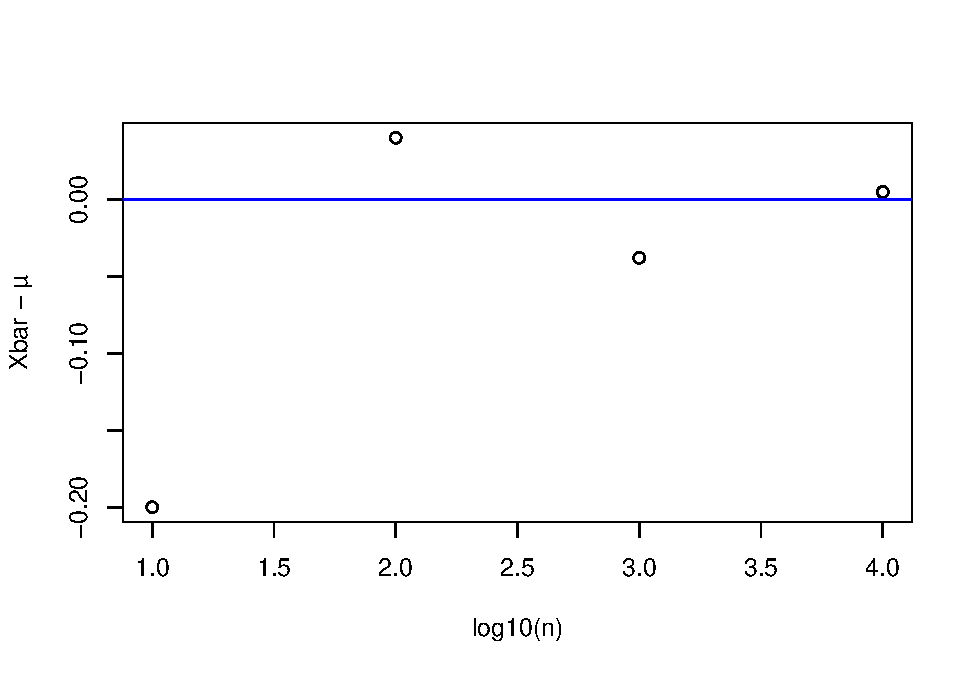
\includegraphics{stad80a1_files/figure-latex/unnamed-chunk-5-1.pdf}

As we can see from the plot above, Xbar-mu is converging to 0 as n goes
to infinity. for small n, we see that xbar-mu deviates from 0. However,
as n increases, the plot gets increasingly closer to near 0.

\hypertarget{b}{%
\subsection{3.b)}\label{b}}

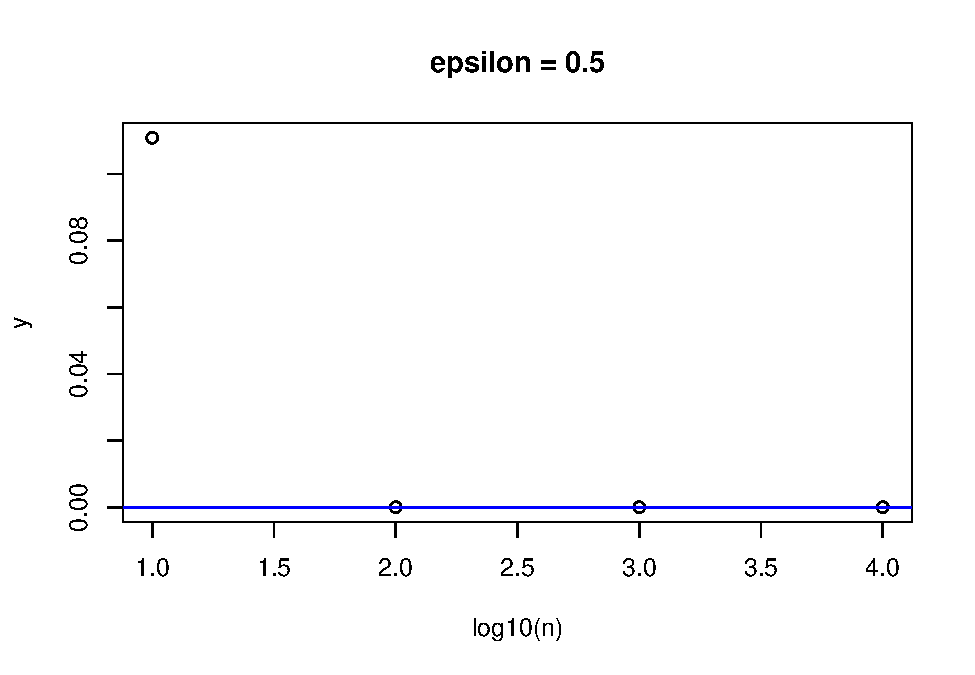
\includegraphics{stad80a1_files/figure-latex/unnamed-chunk-6-1.pdf}
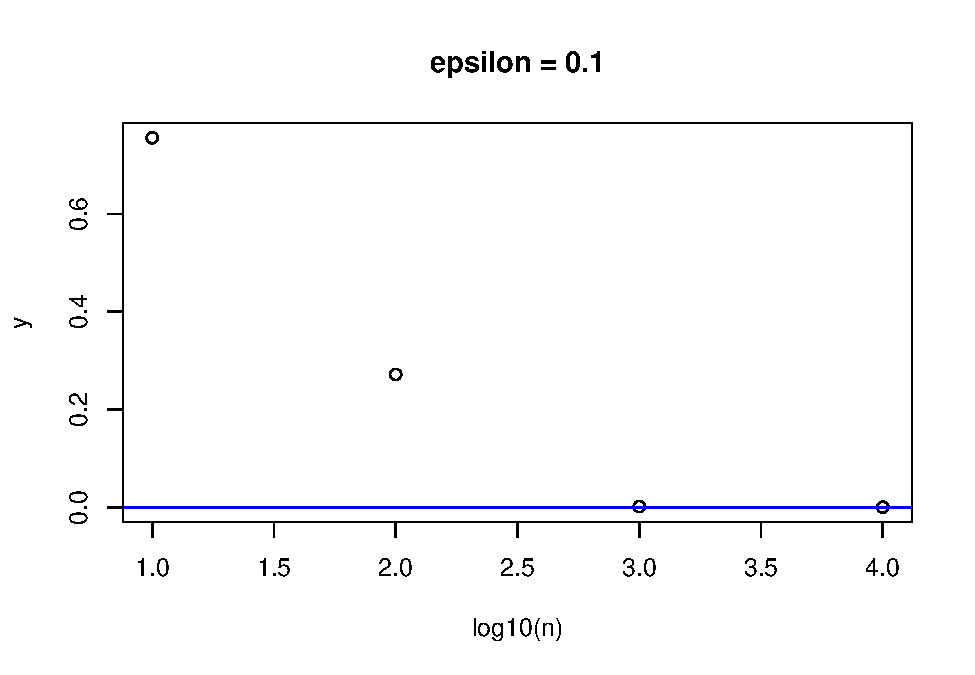
\includegraphics{stad80a1_files/figure-latex/unnamed-chunk-7-1.pdf}
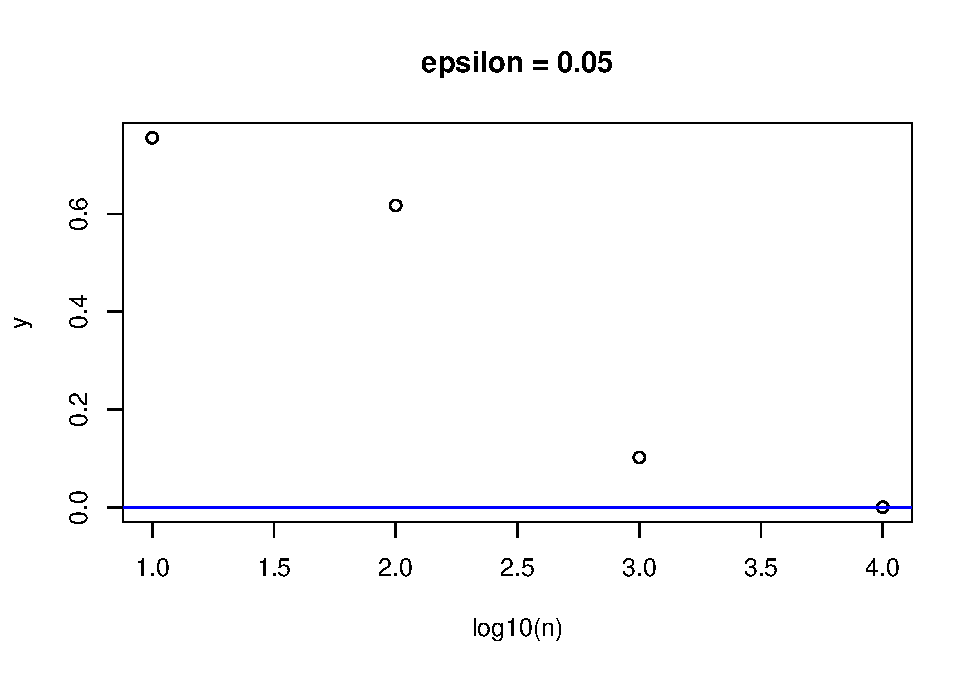
\includegraphics{stad80a1_files/figure-latex/unnamed-chunk-8-1.pdf}

The plots above illustrates the law of large numbers. As n increases
from 10 to 10000, we can see that the data points fall much closer to
the mean(mu), 0 for each of the three plots. We can also see that as
epsilon becomes smaller, the data points for smaller n's tend to be
further away from mu, however they still all will converge to mu with
large n.

\hypertarget{c}{%
\subsection{3.c)}\label{c}}

\begin{Shaded}
\begin{Highlighting}[]
\CommentTok{#install.packages("car")}
\KeywordTok{library}\NormalTok{(car)}
\end{Highlighting}
\end{Shaded}

\begin{verbatim}
## Warning: package 'car' was built under R version 4.0.3
\end{verbatim}

\begin{verbatim}
## Loading required package: carData
\end{verbatim}

\begin{verbatim}
## Warning: package 'carData' was built under R version 4.0.3
\end{verbatim}

\begin{Shaded}
\begin{Highlighting}[]
\KeywordTok{set.seed}\NormalTok{(}\DecValTok{1003643587}\NormalTok{)}
\NormalTok{mu <-}\StringTok{ }\DecValTok{0}
\CommentTok{# var(x) = E(X^2) = 1}
\CommentTok{# sigma^2 = 1}
\NormalTok{sigma <-}\StringTok{ }\DecValTok{1}
\NormalTok{mean10 <-}\StringTok{ }\KeywordTok{c}\NormalTok{()}
\NormalTok{mean100 <-}\StringTok{ }\KeywordTok{c}\NormalTok{()}
\NormalTok{mean1000 <-}\StringTok{ }\KeywordTok{c}\NormalTok{()}
\NormalTok{mean10000 <-}\StringTok{ }\KeywordTok{c}\NormalTok{()}
\ControlFlowTok{for}\NormalTok{ (i }\ControlFlowTok{in} \DecValTok{1}\OperatorTok{:}\DecValTok{10000}\NormalTok{) \{}
\NormalTok{  mean10 <-}\StringTok{ }\KeywordTok{append}\NormalTok{(mean10, }\KeywordTok{sum}\NormalTok{(}\KeywordTok{samples}\NormalTok{(}\DecValTok{10}\NormalTok{))}\OperatorTok{/}\DecValTok{10}\NormalTok{)}
\NormalTok{  mean100 <-}\StringTok{ }\KeywordTok{append}\NormalTok{(mean100, }\KeywordTok{sum}\NormalTok{(}\KeywordTok{samples}\NormalTok{(}\DecValTok{100}\NormalTok{))}\OperatorTok{/}\DecValTok{100}\NormalTok{)}
\NormalTok{  mean1000 <-}\StringTok{ }\KeywordTok{append}\NormalTok{(mean1000, }\KeywordTok{sum}\NormalTok{(}\KeywordTok{samples}\NormalTok{(}\DecValTok{1000}\NormalTok{))}\OperatorTok{/}\DecValTok{1000}\NormalTok{)}
\NormalTok{  mean10000 <-}\StringTok{ }\KeywordTok{append}\NormalTok{(mean10000, }\KeywordTok{sum}\NormalTok{(}\KeywordTok{samples}\NormalTok{(}\DecValTok{10000}\NormalTok{))}\OperatorTok{/}\DecValTok{10000}\NormalTok{)}
\NormalTok{\}}
\end{Highlighting}
\end{Shaded}

n = 10

\begin{Shaded}
\begin{Highlighting}[]
\NormalTok{hist10 <-}\StringTok{ }\KeywordTok{sqrt}\NormalTok{(}\DecValTok{10}\NormalTok{)}\OperatorTok{*}\NormalTok{mean10}\OperatorTok{/}\NormalTok{sigma}
\KeywordTok{hist}\NormalTok{(hist10)}
\end{Highlighting}
\end{Shaded}

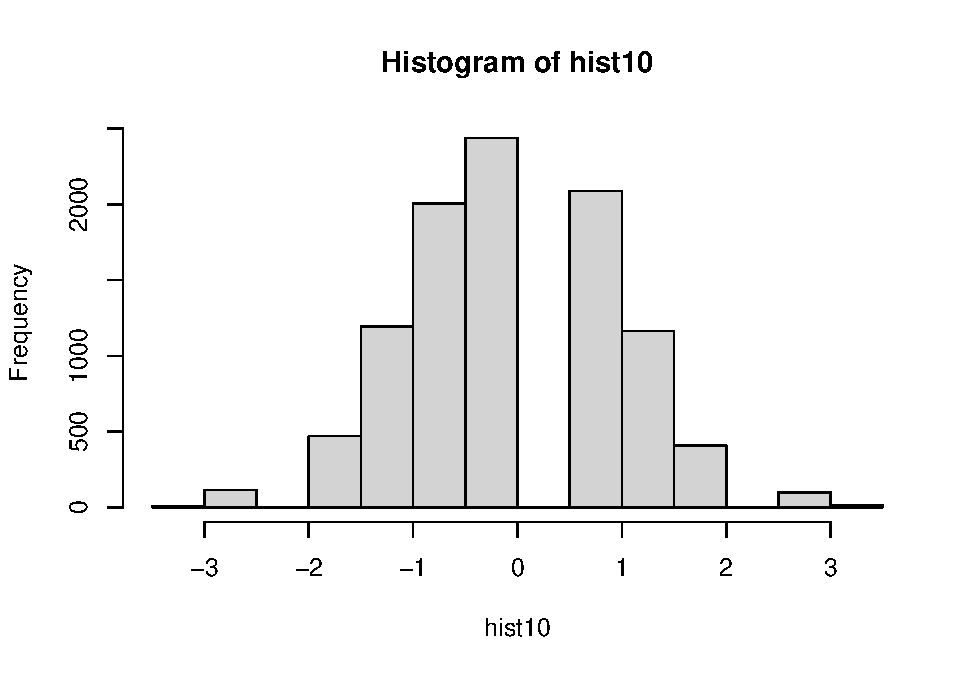
\includegraphics{stad80a1_files/figure-latex/unnamed-chunk-11-1.pdf}

\begin{Shaded}
\begin{Highlighting}[]
\KeywordTok{qqPlot}\NormalTok{(hist10)}
\end{Highlighting}
\end{Shaded}

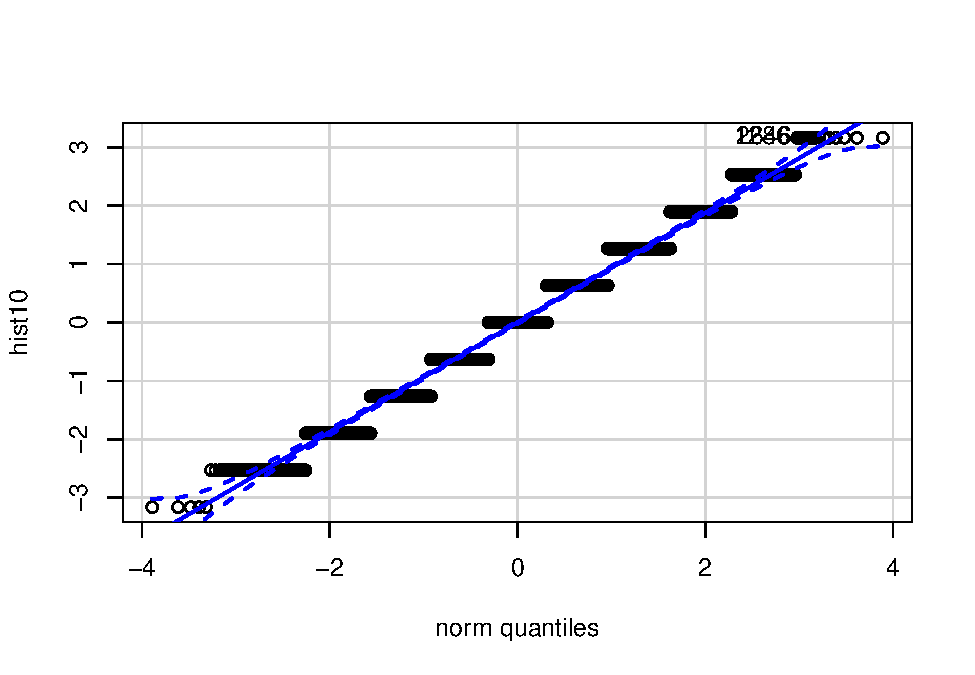
\includegraphics{stad80a1_files/figure-latex/unnamed-chunk-11-2.pdf}

\begin{verbatim}
## [1] 1286 2646
\end{verbatim}

n = 1000

\begin{Shaded}
\begin{Highlighting}[]
\NormalTok{hist1000 <-}\StringTok{ }\KeywordTok{sqrt}\NormalTok{(}\DecValTok{1000}\NormalTok{)}\OperatorTok{*}\NormalTok{mean1000}\OperatorTok{/}\NormalTok{sigma}
\KeywordTok{hist}\NormalTok{(hist1000)}
\end{Highlighting}
\end{Shaded}

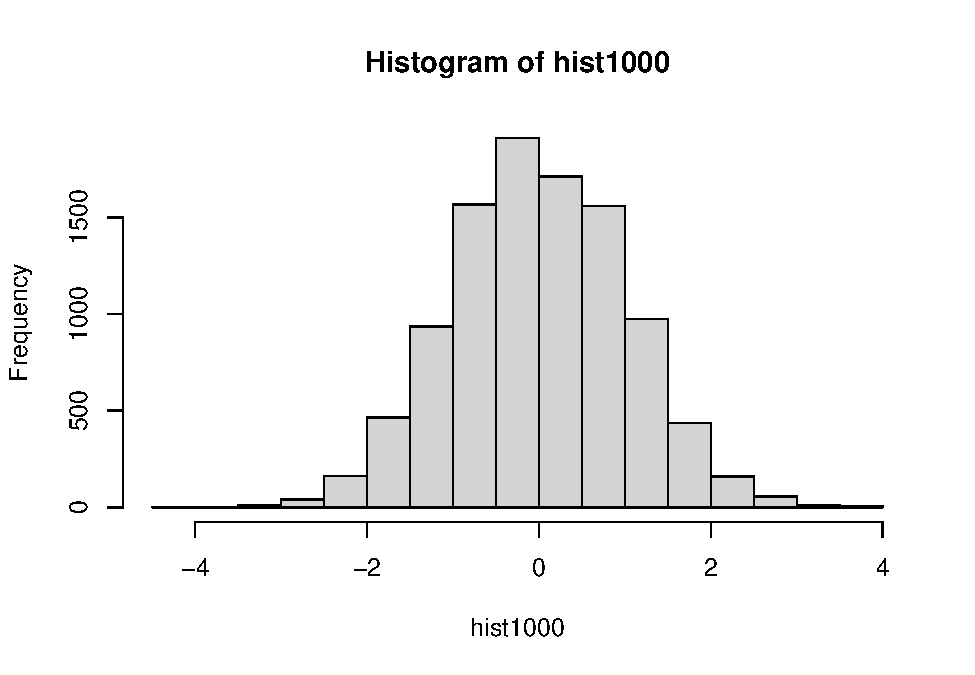
\includegraphics{stad80a1_files/figure-latex/unnamed-chunk-12-1.pdf}

\begin{Shaded}
\begin{Highlighting}[]
\KeywordTok{qqPlot}\NormalTok{(hist1000)}
\end{Highlighting}
\end{Shaded}

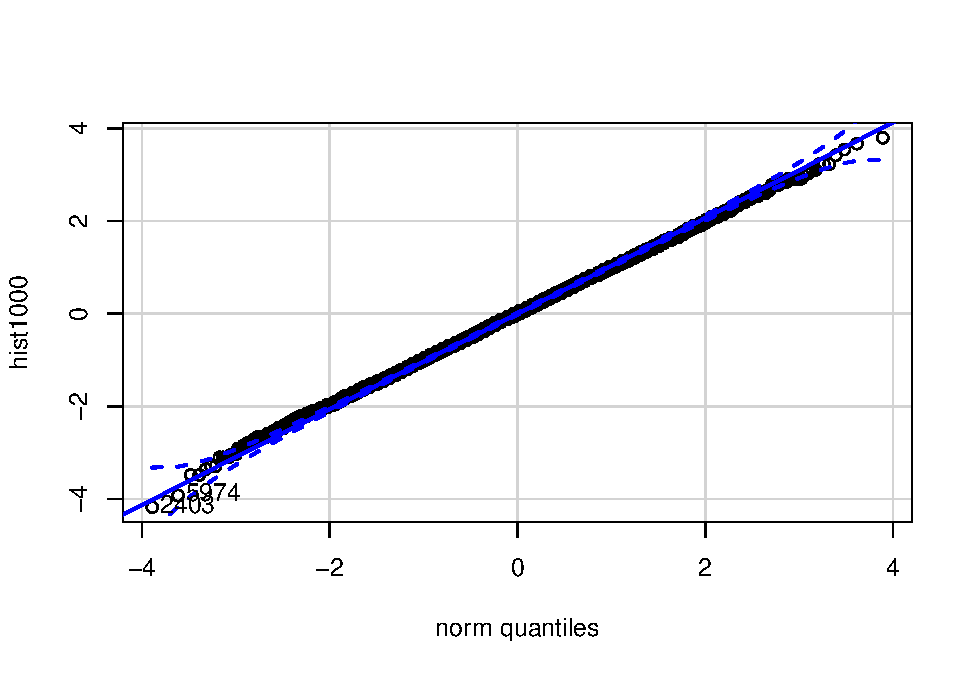
\includegraphics{stad80a1_files/figure-latex/unnamed-chunk-12-2.pdf}

\begin{verbatim}
## [1] 2403 5974
\end{verbatim}

n = 10000

\begin{Shaded}
\begin{Highlighting}[]
\NormalTok{hist10000 <-}\StringTok{ }\KeywordTok{sqrt}\NormalTok{(}\DecValTok{10000}\NormalTok{)}\OperatorTok{*}\NormalTok{mean10000}\OperatorTok{/}\NormalTok{sigma}
\KeywordTok{hist}\NormalTok{(hist10000)}
\end{Highlighting}
\end{Shaded}

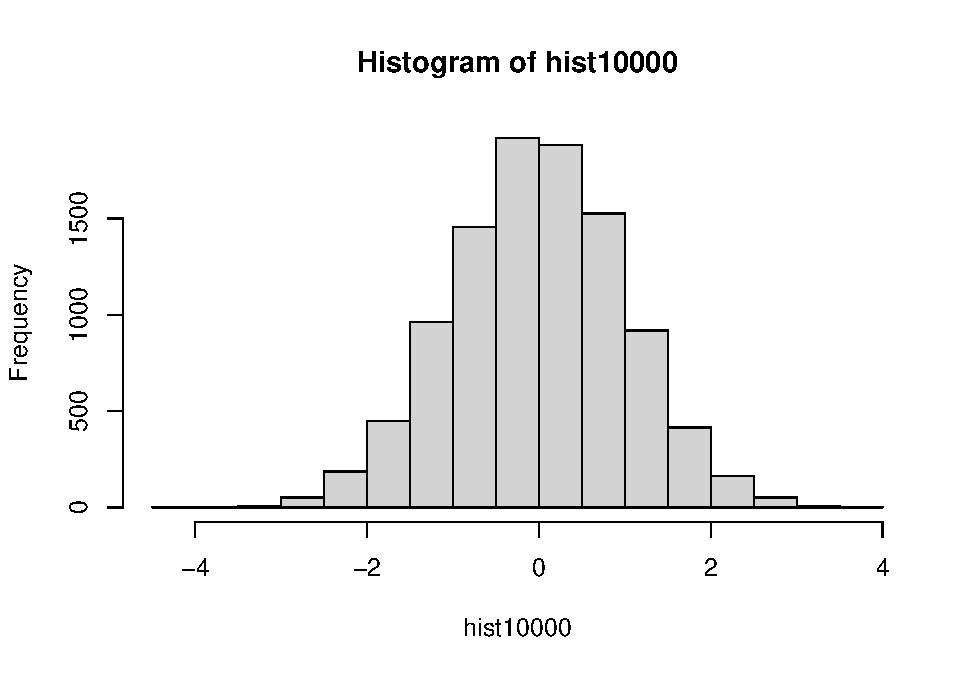
\includegraphics{stad80a1_files/figure-latex/unnamed-chunk-13-1.pdf}

\begin{Shaded}
\begin{Highlighting}[]
\KeywordTok{qqPlot}\NormalTok{(hist10000)}
\end{Highlighting}
\end{Shaded}

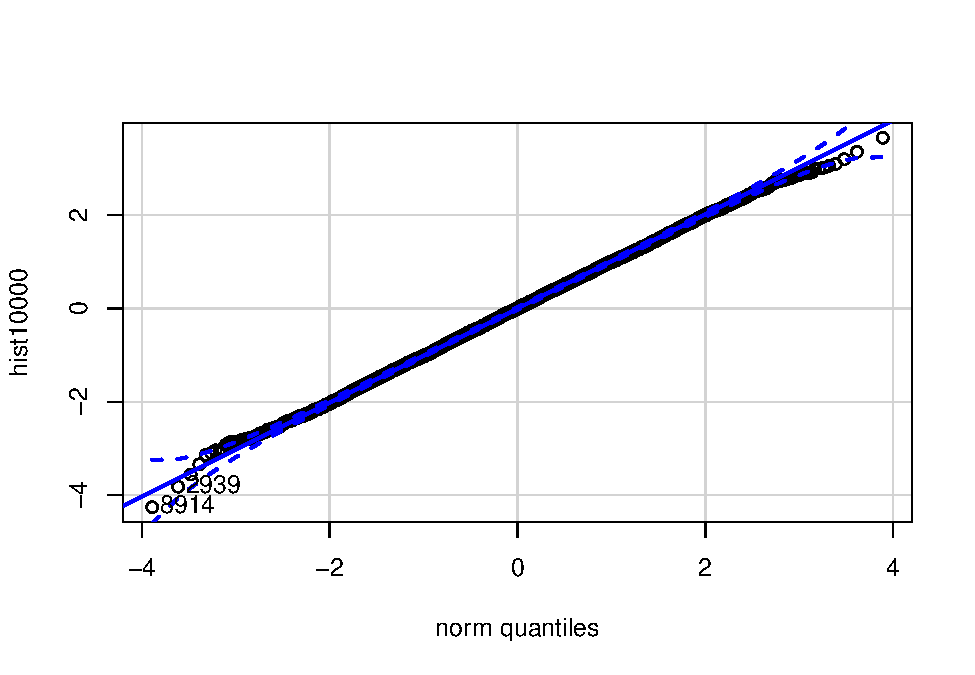
\includegraphics{stad80a1_files/figure-latex/unnamed-chunk-13-2.pdf}

\begin{verbatim}
## [1] 8914 2939
\end{verbatim}

As we can see from the QQ plots and histograms, as n increases we can
see that the data is more like standard normal. The histograms look more
like normal as n increases and the qq plots are more linear with less
outliers. These plots also show the Central Limit Theorem as we have mu
= E(x) and simga\^{}2 = var(x). As n approaches infinity, sqrt(n)(xbar -
mu)/sigma approaches the standard normal in distribution.\\
\#\# 3.d)

\begin{Shaded}
\begin{Highlighting}[]
\NormalTok{averag <-}\StringTok{ }\ControlFlowTok{function}\NormalTok{(data, e) \{}
\NormalTok{  data <-}\StringTok{ }\KeywordTok{abs}\NormalTok{(data)}
\NormalTok{  data <-}\StringTok{ }\KeywordTok{replace}\NormalTok{(data, data }\OperatorTok{>}\StringTok{ }\NormalTok{e, }\DecValTok{1}\NormalTok{)}
\NormalTok{  data <-}\StringTok{ }\KeywordTok{replace}\NormalTok{(data, data }\OperatorTok{<=}\StringTok{ }\NormalTok{e, }\DecValTok{0}\NormalTok{)}
  \KeywordTok{return}\NormalTok{(data)}
\NormalTok{\}}
\end{Highlighting}
\end{Shaded}

\begin{Shaded}
\begin{Highlighting}[]
\NormalTok{logVals =}\StringTok{ }\KeywordTok{c}\NormalTok{(}\KeywordTok{log}\NormalTok{(}\DecValTok{10}\NormalTok{, }\DataTypeTok{base =} \DecValTok{10}\NormalTok{), }\KeywordTok{log}\NormalTok{(}\DecValTok{100}\NormalTok{, }\DataTypeTok{base =} \DecValTok{10}\NormalTok{), }\KeywordTok{log}\NormalTok{(}\DecValTok{1000}\NormalTok{, }\DataTypeTok{base =} \DecValTok{10}\NormalTok{), }\KeywordTok{log}\NormalTok{(}\DecValTok{10000}\NormalTok{, }\DataTypeTok{base =} \DecValTok{10}\NormalTok{))}
\NormalTok{Y10 <-}\StringTok{ }\KeywordTok{rnorm}\NormalTok{(}\DecValTok{10}\NormalTok{,}\DecValTok{0}\NormalTok{,}\DecValTok{1}\NormalTok{)}
\NormalTok{Y100 <-}\StringTok{ }\KeywordTok{rnorm}\NormalTok{(}\DecValTok{100}\NormalTok{,}\DecValTok{0}\NormalTok{,}\DecValTok{1}\NormalTok{)}
\NormalTok{Y1000 <-}\StringTok{ }\KeywordTok{rnorm}\NormalTok{(}\DecValTok{1000}\NormalTok{,}\DecValTok{0}\NormalTok{,}\DecValTok{1}\NormalTok{)}
\NormalTok{Y10000 <-}\StringTok{ }\KeywordTok{rnorm}\NormalTok{(}\DecValTok{10000}\NormalTok{,}\DecValTok{0}\NormalTok{,}\DecValTok{1}\NormalTok{)}
\NormalTok{data10 <-}\StringTok{ }\KeywordTok{sqrt}\NormalTok{(}\DecValTok{10}\NormalTok{)}\OperatorTok{*}\NormalTok{mean10 }\OperatorTok{-}\StringTok{ }\NormalTok{Y10}
\NormalTok{data10 <-}\StringTok{ }\KeywordTok{averag}\NormalTok{(data10, }\FloatTok{0.001}\NormalTok{)}
\NormalTok{data100 <-}\StringTok{ }\KeywordTok{sqrt}\NormalTok{(}\DecValTok{100}\NormalTok{)}\OperatorTok{*}\NormalTok{mean100 }\OperatorTok{-}\StringTok{ }\NormalTok{Y100}
\NormalTok{data100 <-}\StringTok{ }\KeywordTok{averag}\NormalTok{(data100, }\FloatTok{0.001}\NormalTok{)}
\NormalTok{data1000 <-}\StringTok{ }\KeywordTok{sqrt}\NormalTok{(}\DecValTok{1000}\NormalTok{)}\OperatorTok{*}\NormalTok{mean1000 }\OperatorTok{-}\StringTok{ }\NormalTok{Y1000}
\NormalTok{data1000 <-}\StringTok{ }\KeywordTok{averag}\NormalTok{(data1000, }\FloatTok{0.001}\NormalTok{)}
\NormalTok{data10000 <-}\StringTok{ }\KeywordTok{sqrt}\NormalTok{(}\DecValTok{10000}\NormalTok{)}\OperatorTok{*}\NormalTok{mean10000 }\OperatorTok{-}\StringTok{ }\NormalTok{Y10000}
\NormalTok{data10000 <-}\StringTok{ }\KeywordTok{averag}\NormalTok{(data10000, }\FloatTok{0.001}\NormalTok{)}
\NormalTok{plotData <-}\StringTok{ }\KeywordTok{c}\NormalTok{(}\KeywordTok{mean}\NormalTok{(data10), }\KeywordTok{mean}\NormalTok{(data100), }\KeywordTok{mean}\NormalTok{(data1000), }\KeywordTok{mean}\NormalTok{(data10000))}
\KeywordTok{plot}\NormalTok{(logVals, plotData)}
\end{Highlighting}
\end{Shaded}

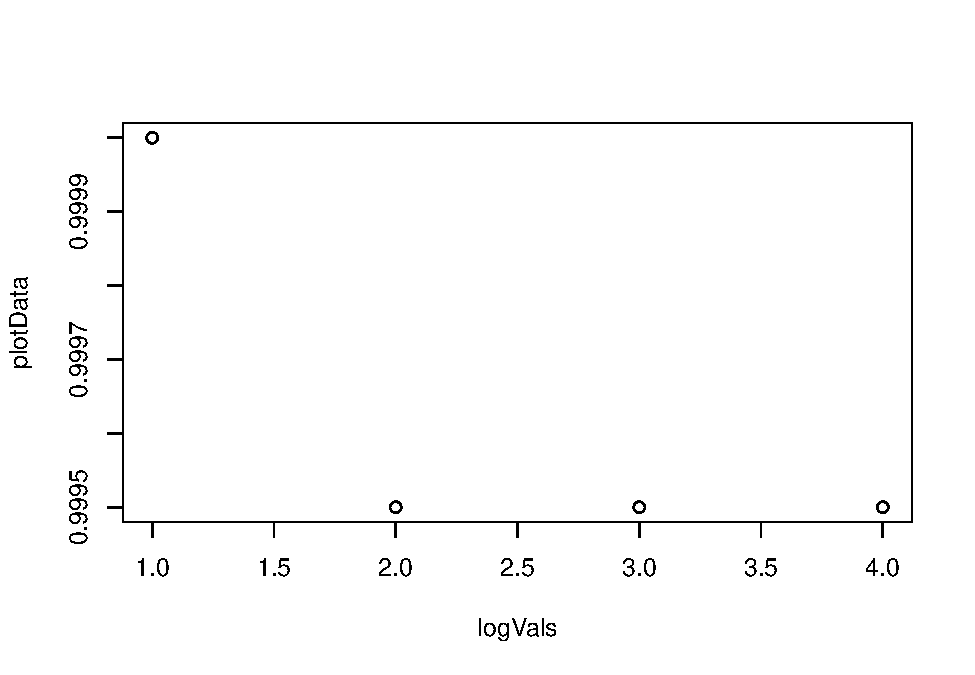
\includegraphics{stad80a1_files/figure-latex/unnamed-chunk-15-1.pdf}

From the plot above, we see that it does not converge to Y in
probability because even as n increases, the values do not necessarily
approach 0. They still converge in distribution but this does not mean
that all the values will be converging. As the standardized values of x
approaches y in distribution, but not in probability.

\hypertarget{section-4}{%
\section{4.}\label{section-4}}

\hypertarget{a-2}{%
\subsection{4.a)}\label{a-2}}

\begin{Shaded}
\begin{Highlighting}[]
\CommentTok{#install.packages("bigmemory")}
\KeywordTok{library}\NormalTok{(bigmemory)}
\end{Highlighting}
\end{Shaded}

\begin{verbatim}
## Warning: package 'bigmemory' was built under R version 4.0.3
\end{verbatim}

\begin{Shaded}
\begin{Highlighting}[]
\NormalTok{X <-}\StringTok{ }\KeywordTok{read.big.matrix}\NormalTok{(}\StringTok{"ratings.dat"}\NormalTok{, }\DataTypeTok{type =} \StringTok{"integer"}\NormalTok{, }\DataTypeTok{col.names =} \KeywordTok{c}\NormalTok{(}\StringTok{"UserID"}\NormalTok{, }\StringTok{"ProfileID"}\NormalTok{, }\StringTok{"Rating"}\NormalTok{))}
\KeywordTok{head}\NormalTok{(X)}
\end{Highlighting}
\end{Shaded}

\begin{verbatim}
##      UserID ProfileID Rating
## [1,]  56669     39491      6
## [2,]  56919      8035     10
## [3,] 108853    102321     10
## [4,] 116784     52568      2
## [5,] 132748    220878     10
## [6,] 120139     29077      9
\end{verbatim}

\begin{Shaded}
\begin{Highlighting}[]
\NormalTok{  RatingAll <-}\StringTok{ }\NormalTok{X[, }\DecValTok{3}\NormalTok{]}
\NormalTok{  C <-}\StringTok{ }\KeywordTok{sum}\NormalTok{(RatingAll)}\OperatorTok{/}\DecValTok{3000000}
\end{Highlighting}
\end{Shaded}

\begin{Shaded}
\begin{Highlighting}[]
\NormalTok{weighted.rank <-}\StringTok{ }\ControlFlowTok{function}\NormalTok{(ProfileID) \{}
\NormalTok{  byProfile <-}\StringTok{ }\KeywordTok{mwhich}\NormalTok{(X, }\StringTok{"ProfileID"}\NormalTok{, ProfileID, }\StringTok{"eq"}\NormalTok{)}
\NormalTok{  newX <-}\StringTok{ }\NormalTok{X[byProfile, ]}
\NormalTok{  byRating <-}\StringTok{ }\NormalTok{newX[, }\DecValTok{3}\NormalTok{]}
\NormalTok{  v <-}\StringTok{ }\KeywordTok{length}\NormalTok{(byRating)}
\NormalTok{  R <-}\StringTok{ }\KeywordTok{sum}\NormalTok{(byRating)}\OperatorTok{/}\NormalTok{v}
\NormalTok{  m <-}\StringTok{ }\DecValTok{4182}
\NormalTok{  weightedRank <-}\StringTok{ }\NormalTok{((v}\OperatorTok{/}\NormalTok{(v}\OperatorTok{+}\NormalTok{m))}\OperatorTok{*}\NormalTok{R)}\OperatorTok{+}\NormalTok{((m}\OperatorTok{/}\NormalTok{(v}\OperatorTok{+}\NormalTok{m))}\OperatorTok{*}\NormalTok{C)}
  \KeywordTok{return}\NormalTok{(weightedRank)}
\NormalTok{\}}
\KeywordTok{weighted.rank}\NormalTok{(}\DecValTok{39491}\NormalTok{)}
\end{Highlighting}
\end{Shaded}

\begin{verbatim}
## [1] 5.977027
\end{verbatim}

\begin{Shaded}
\begin{Highlighting}[]
\NormalTok{byUser <-}\StringTok{ }\KeywordTok{mwhich}\NormalTok{(X, }\StringTok{"UserID"}\NormalTok{, }\DecValTok{100}\NormalTok{, }\StringTok{"eq"}\NormalTok{)}
\NormalTok{byUser <-}\StringTok{ }\NormalTok{X[byUser, ]}
\NormalTok{byUser <-}\StringTok{ }\NormalTok{byUser[, }\DecValTok{2}\NormalTok{]}
\NormalTok{eachProfile <-}\StringTok{ }\KeywordTok{lapply}\NormalTok{(byUser, weighted.rank)}
\NormalTok{plotData <-}\StringTok{ }\KeywordTok{unlist}\NormalTok{(eachProfile)}
\KeywordTok{hist}\NormalTok{(plotData, }\DataTypeTok{main =} \StringTok{"weighted ranks of all profiles rated by UserID 100"}\NormalTok{, }\DataTypeTok{xlab =} \StringTok{"weighted rank"}\NormalTok{)}
\end{Highlighting}
\end{Shaded}

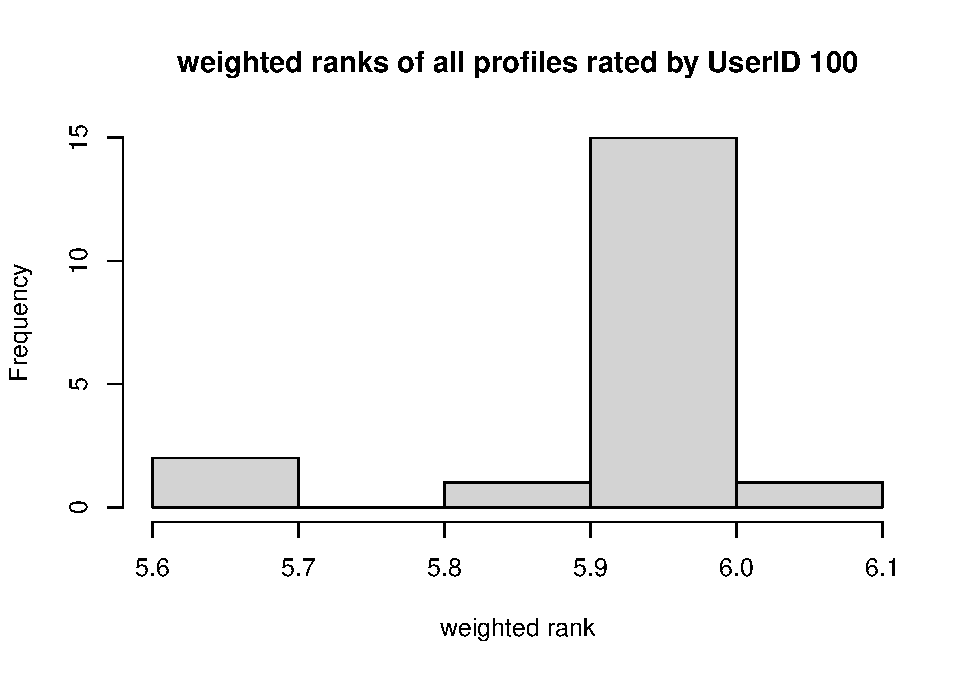
\includegraphics{stad80a1_files/figure-latex/unnamed-chunk-19-1.pdf}

\hypertarget{b-1}{%
\subsection{4.b)}\label{b-1}}

\begin{Shaded}
\begin{Highlighting}[]
\KeywordTok{load}\NormalTok{(}\StringTok{"users.Rdata"}\NormalTok{)}
\end{Highlighting}
\end{Shaded}

\begin{enumerate}
\def\labelenumi{\arabic{enumi})}
\tightlist
\item
  male users coming from New York State, State==New York
\end{enumerate}

\begin{Shaded}
\begin{Highlighting}[]
\NormalTok{ratingsM <-}\StringTok{ }\KeywordTok{c}\NormalTok{()}
\NormalTok{newYorkM <-}\StringTok{ }\NormalTok{User[}\KeywordTok{which}\NormalTok{(User}\OperatorTok{$}\NormalTok{Gender }\OperatorTok{==}\StringTok{ 'M'} \OperatorTok{&}\StringTok{ }\NormalTok{User}\OperatorTok{$}\NormalTok{State }\OperatorTok{==}\StringTok{ 'New York'}\NormalTok{), ]}
\NormalTok{newYorkM <-}\StringTok{ }\NormalTok{newYorkM[ , }\DecValTok{1}\NormalTok{]}
\ControlFlowTok{for}\NormalTok{(i }\ControlFlowTok{in}\NormalTok{ newYorkM) \{}
\NormalTok{  byUser <-}\StringTok{ }\KeywordTok{mwhich}\NormalTok{(X, }\StringTok{"UserID"}\NormalTok{, i, }\StringTok{"eq"}\NormalTok{)}
\NormalTok{  byUser <-}\StringTok{ }\NormalTok{X[byUser, ]}
  \ControlFlowTok{if}\NormalTok{(}\KeywordTok{identical}\NormalTok{(}\KeywordTok{nrow}\NormalTok{(byUser), }\OtherTok{NULL}\NormalTok{))\{}
\NormalTok{    byUser <-}\StringTok{ }\NormalTok{byUser[}\DecValTok{3}\NormalTok{]}
\NormalTok{    ratingsM <-}\StringTok{ }\KeywordTok{append}\NormalTok{(ratingsM, byUser)}
\NormalTok{  \} }\ControlFlowTok{else}\NormalTok{ \{}
\NormalTok{    byUser <-}\StringTok{ }\NormalTok{byUser[ , }\DecValTok{3}\NormalTok{]}
\NormalTok{    ratingsM <-}\StringTok{ }\KeywordTok{append}\NormalTok{(ratingsM, byUser)}
\NormalTok{  \}}
\NormalTok{\}}
\end{Highlighting}
\end{Shaded}

\begin{enumerate}
\def\labelenumi{\arabic{enumi})}
\setcounter{enumi}{1}
\tightlist
\item
  female users coming from California, State==CA
\end{enumerate}

\begin{Shaded}
\begin{Highlighting}[]
\NormalTok{ratingsF <-}\StringTok{ }\KeywordTok{c}\NormalTok{()}
\NormalTok{CAF <-}\StringTok{ }\NormalTok{User[}\KeywordTok{which}\NormalTok{(User}\OperatorTok{$}\NormalTok{Gender }\OperatorTok{==}\StringTok{ 'F'} \OperatorTok{&}\StringTok{ }\NormalTok{User}\OperatorTok{$}\NormalTok{State }\OperatorTok{==}\StringTok{ 'CA'}\NormalTok{), ]}
\NormalTok{CAF <-}\StringTok{ }\NormalTok{CAF[ , }\DecValTok{1}\NormalTok{]}
\ControlFlowTok{for}\NormalTok{(i }\ControlFlowTok{in}\NormalTok{ CAF) \{}
\NormalTok{  byUser <-}\StringTok{ }\KeywordTok{mwhich}\NormalTok{(X, }\StringTok{"UserID"}\NormalTok{, i, }\StringTok{"eq"}\NormalTok{)}
\NormalTok{  byUser <-}\StringTok{ }\NormalTok{X[byUser, ]}
  \ControlFlowTok{if}\NormalTok{(}\KeywordTok{identical}\NormalTok{(}\KeywordTok{nrow}\NormalTok{(byUser), }\OtherTok{NULL}\NormalTok{))\{}
\NormalTok{    byUser <-}\StringTok{ }\NormalTok{byUser[}\DecValTok{3}\NormalTok{]}
\NormalTok{    ratingsF <-}\StringTok{ }\KeywordTok{append}\NormalTok{(ratingsF, byUser)}
\NormalTok{  \} }\ControlFlowTok{else}\NormalTok{ \{}
\NormalTok{    byUser <-}\StringTok{ }\NormalTok{byUser[ , }\DecValTok{3}\NormalTok{]}
\NormalTok{    ratingsF <-}\StringTok{ }\KeywordTok{append}\NormalTok{(ratingsF, byUser)}
\NormalTok{  \}}
\NormalTok{\}}
\end{Highlighting}
\end{Shaded}

\begin{Shaded}
\begin{Highlighting}[]
\NormalTok{z <-}\StringTok{ }\KeywordTok{c}\NormalTok{(}\StringTok{"ratingsM"}\NormalTok{, }\StringTok{"ratingsF"}\NormalTok{)}
\NormalTok{histData <-}\StringTok{ }\KeywordTok{lapply}\NormalTok{(z, get, }\DataTypeTok{envir=}\KeywordTok{environment}\NormalTok{())}
\KeywordTok{names}\NormalTok{(histData) <-}\StringTok{ }\NormalTok{z}
\KeywordTok{boxplot}\NormalTok{(histData)}
\end{Highlighting}
\end{Shaded}

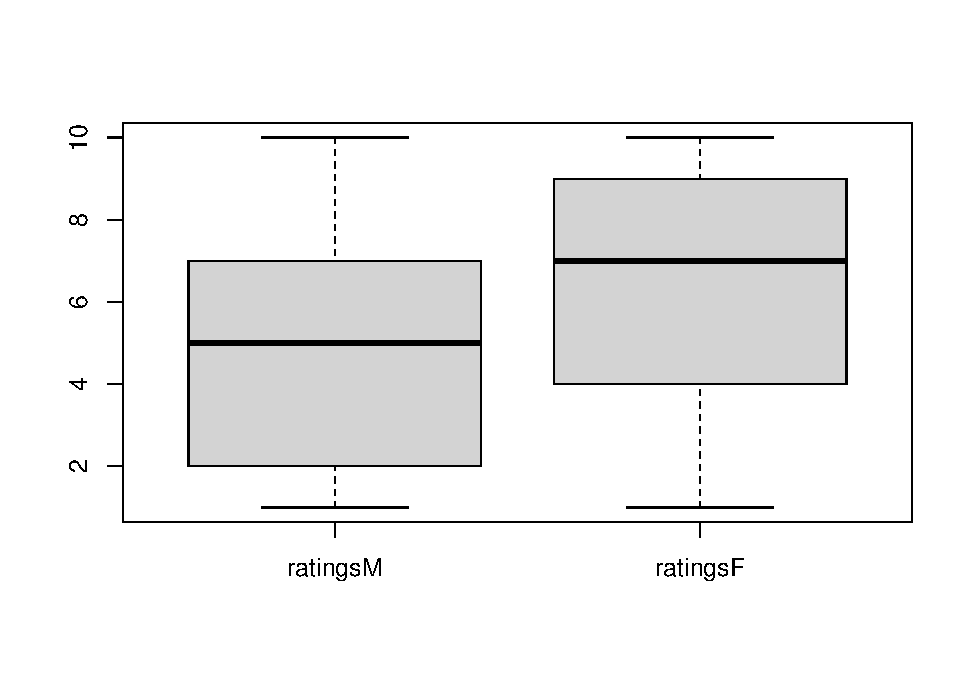
\includegraphics{stad80a1_files/figure-latex/unnamed-chunk-23-1.pdf}

Above is a boxplot of ratings of Males from New York, against ratings of
Females from CA

\hypertarget{c-1}{%
\subsection{4.c)}\label{c-1}}

\begin{Shaded}
\begin{Highlighting}[]
\CommentTok{#install.packages("biganalytics")}
\KeywordTok{library}\NormalTok{(biganalytics)}
\end{Highlighting}
\end{Shaded}

\begin{verbatim}
## Warning: package 'biganalytics' was built under R version 4.0.3
\end{verbatim}

\begin{verbatim}
## Loading required package: foreach
\end{verbatim}

\begin{verbatim}
## Warning: package 'foreach' was built under R version 4.0.3
\end{verbatim}

\begin{verbatim}
## Loading required package: biglm
\end{verbatim}

\begin{verbatim}
## Warning: package 'biglm' was built under R version 4.0.3
\end{verbatim}

\begin{verbatim}
## Loading required package: DBI
\end{verbatim}

\begin{verbatim}
## Warning: package 'DBI' was built under R version 4.0.3
\end{verbatim}

\begin{Shaded}
\begin{Highlighting}[]
\KeywordTok{head}\NormalTok{(X)}
\end{Highlighting}
\end{Shaded}

\begin{verbatim}
##      UserID ProfileID Rating
## [1,]  56669     39491      6
## [2,]  56919      8035     10
## [3,] 108853    102321     10
## [4,] 116784     52568      2
## [5,] 132748    220878     10
## [6,] 120139     29077      9
\end{verbatim}

N=3000000 \# number of rating records Nu=135359 \# maximum of UserID
Np=220970 \# maximum of ProfileID user.rat=rep(0,Nu) \# user.rat{[}i{]}
denotes the sum of ratings given by user i user.num=rep(0,Nu) \#
user.num{[}i{]} denotes the number of ratings given by user i
profile.rat=rep(0,Np) \# profile.rat{[}i{]} denotes the sum of ratings
given to profile i profile.num=rep(0,Np) \# user.rat{[}i{]} denotes the
number of ratings given to profile i for (i in 1:N)\{ \# In each
iteration, we update the four arrays, i.e.~user.rat, user.num,
profile.rat, profile.num, using one rating record.
user.rat{[}X{[}i,`UserID'{]}{]}=user.rat{[}X{[}i,`UserID'{]}{]}+X{[}i,`Rating'{]}
\# The matrix X here comes from the file `ratings.dat'
user.num{[}X{[}i,`UserID'{]}{]}=user.num{[}X{[}i,`UserID'{]}{]}+1
profile.rat{[}X{[}i,`ProfileID'{]}{]}=profile.rat{[}X{[}i,`ProfileID'{]}{]}+X{[}i,`Rating'{]}
profile.num{[}X{[}i,`ProfileID'{]}{]}=profile.num{[}X{[}i,`ProfileID'{]}{]}+1
if (i \%\% 10000==0) print(i/10000) \} user.ave=user.rat/user.num
profile.ave=profile.rat/profile.num X1=big.matrix(nrow=nrow(X),
ncol=ncol(X), type= ``double'', dimnames=list(NULL,
c(`UsrAveRat',`PrfAveRat',`Rat'))) X1{[},`Rat'{]}=X{[},`Rating'{]}
X1{[},`UsrAveRat'{]}=user.ave{[}X{[},'UserID'{]}{]}
X1{[},`PrfAveRat'{]}=profile.ave{[}X{[},'ProfileID'{]}{]} \# X1 is the
new data matrix we will work with in regression. user.ave profile.ave

\end{document}
